\section{Methodology}

\subsection{N-Dimension Matrix}
\begin{frame}
  \frametitle{N-dimension Matrix}
  \framesubtitle{STL containers}
  STL provides containers \texttt{std::array} and \texttt{std::vector} for creating one-dimension array.
  \\
  There are two way for dealing with high-dimension data:
  \begin{enumerate}
    \item Nesting the one dimension arrays or vectors.
    \item Hierarchy approach, designing derived classes of one-dimension array base class.
  \end{enumerate}
  \begin{figure}[htbp]
    \centering
    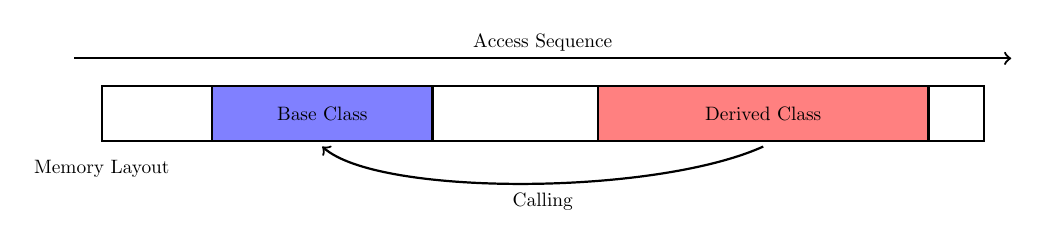
\begin{tikzpicture}[scale=0.7, transform shape]
      % \draw[help lines, step=1] (-10,-2) grid (10,2);    
      % % Draw axes
      % \draw[dashed,->] (-10,0) -- (10,0) node[right] {x};
      % \draw[dashed,->] (0,-2) -- (0,2) node[above] {y};

      \draw[thick, ->] (-8.5, 1.5) -- node[midway, above] {Access Sequence} (8.5, 1.5);

      \draw[thick] (-8,1) rectangle (8,0);
      \node at (-8,-0.5) [] {Memory Layout};

      \draw[thick, fill=blue!50] (-6,1) rectangle (-2,0);
      \node at (-4, 0.5) [] {Base Class};

      \draw[thick, fill=red!50] (1,1) rectangle (7,0);
      \node at (4, 0.5) [] {Derived Class};

      \node at (0, -1.1) [] {Calling};
      \draw[thick, ->] (4, -0.1) 
        .. controls (2, -1) and (-3, -1) .. (-4, -0.1);

    \end{tikzpicture}
    \caption{Derived Class calling members in Base class, timing is not predictable.}
    \label{<label>}
  \end{figure}
\end{frame}


\begin{frame}
  % \frametitle{N-dimension Matrix}
  % \framesubtitle{Memory Layout Problem}
  \begin{enumerate}
    \item Nesting multi-dimension array has non-contiguous memory layout.
    \item Derived class needs more time to access members in base class.
    \item Poor cache utilization leads to poor performance.
    \item MPI type create requires contiguous memory layout.
  \end{enumerate}
  % 插入图
  \begin{figure}[htbp]
    \centering
    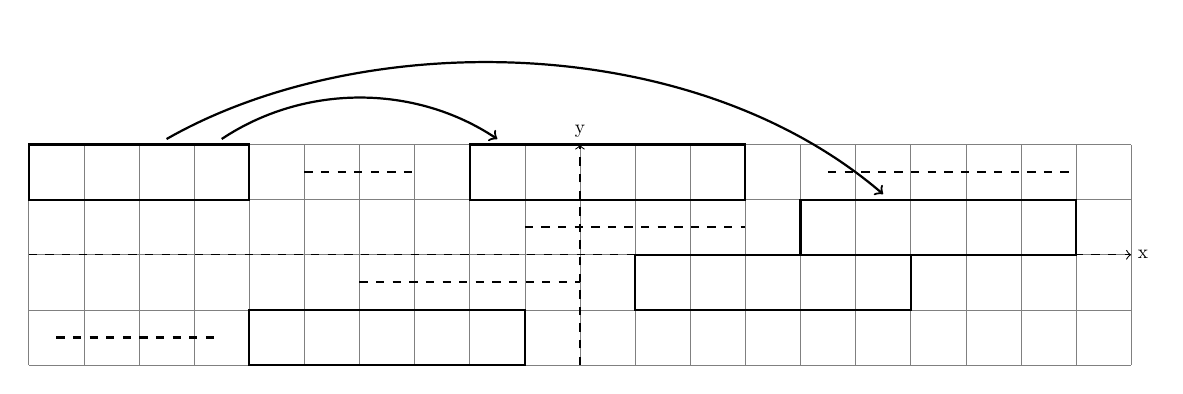
\begin{tikzpicture}[scale=0.7, transform shape]
      \draw[help lines, step=1] (-10,-2) grid (10,2);    
      % Draw axes
      \draw[dashed,->] (-10,0) -- (10,0) node[right] {x};
      \draw[dashed,->] (0,-2) -- (0,2) node[above] {y};

      \draw[thick] (-10,2) rectangle (-6,1);    
      \draw[dashed, thick] (-5,1.5) -- (-3, 1.5);

  
      \draw[thick] (-2,2) rectangle (3,1);
      \draw[dashed, thick] (4.5,1.5) -- (9, 1.5);

      \draw[dashed, thick] (-1,0.5) -- (3, 0.5);
      \draw[thick] (4,1) rectangle (9,0);
      

      \draw[thick] (1,0) rectangle (6,-1);
      \draw[dashed, thick] (-4, -0.5) -- (0, -0.5);

      \draw[dashed, thick] (-9.5, -1.5) -- (-6.5, -1.5);
      \draw[thick] (-6,-1) rectangle (-1,-2);


      \draw[thick, ->] (-6.5, 2.1) 
      .. controls (-5, 3.1) and (-3, 3.1) .. (-1.5, 2.1);

      \draw[thick, ->] (-7.5, 2.1) 
      .. controls (-4, 4.1) and (2, 4.1) .. (5.5, 1.1);
      
    \end{tikzpicture}
    \caption{<caption>}
    \label{<label>}
  \end{figure}
\end{frame}


\begin{frame}
  \frametitle{N-dimension Matrix}
  \framesubtitle{Solution}
  \begin{itemize}
    \item An external small \texttt{\_\_multi\_array\_shape} object defines the routines for accessing the elements.
    \item Smart pointer, ensure memory's contiguous layout and safety.
    \item Separate into two detail and user interface objects adhering RAII rules.
  \end{itemize}


  % 插入图
\end{frame}







\subsection{Parallelization of Multi-dimensional Matrices on cartesian Topologies}


% \section{Implementations}
% \subsection{PDE Solvers}
% % \subsection{General Setups}
% % \subsection{Parallel Strategies}


\subsection{PINN Model}
